\section{Experiments}
\label{sec:exps}

In the following section, we outline the experiments performed to characterize the behavior of our method. First, we compare our method with existing baselines for segmentation purposes. We then perform an ablation study to demonstrate which aspect of our method provides what quantitative benefits, as well as the impact of the class-prior upper-bound initialization. Last, we show how our stopping condition performs in establishing useful class priors.

\subsection{Datasets}
To validate our method, we evaluate it on the publicly available dataset used in~\cite{lejeune18}. It consists of a variety of video and volumes of different modalities with 2D annotation points for different objects of interest, as well as the associated groundtruth segmentations. Specifically, it includes four different subsets of data:
\begin{itemize}
\item \textbf{Brain:} Four 3D T2-weighted MRI scans chosen at random from the publicly available BRATS challenge dataset~\cite{menze15}, where tumors are the object of interest.
\item \textbf{Tweezer:} Four sequences from the training set of the publicly dataset MICCAI Endoscopic Vision challenge: Robotic Instruments segmentation~\cite{endochal}. The surgical instrument is the object to segment in these sequences.
\item \textbf{Slitlamp:} Four slit-lamp video recordings of human retinas, where the optic disk is to be segmented.
\item \textbf{Cochlea:} Four volumes of 3D CT scans of the inner ear, where the cochlea must be annotated. This object is the most challenging object to segment due to its challenging geometry (\ie non-concave shape).
\end{itemize}

\begin{figure*}[t]
\caption{Visualization of stopping conditions for \SSnnPU~method. For each tested image type, we show: (top) Mean Absolute Error (MAE) between the estimated and the true prior, (bottom) Variance of the pseudo-negatives. We also show here threshold (in dashed-red), and the minimum number of epochs (dashed-green). Both the optimal (circle) and the stopping conditions-based class-priors (cross) are shown on each of the sequences of each type (one line per sequence). }
\centering
\begin{tabular}{@{}cc@{}}
    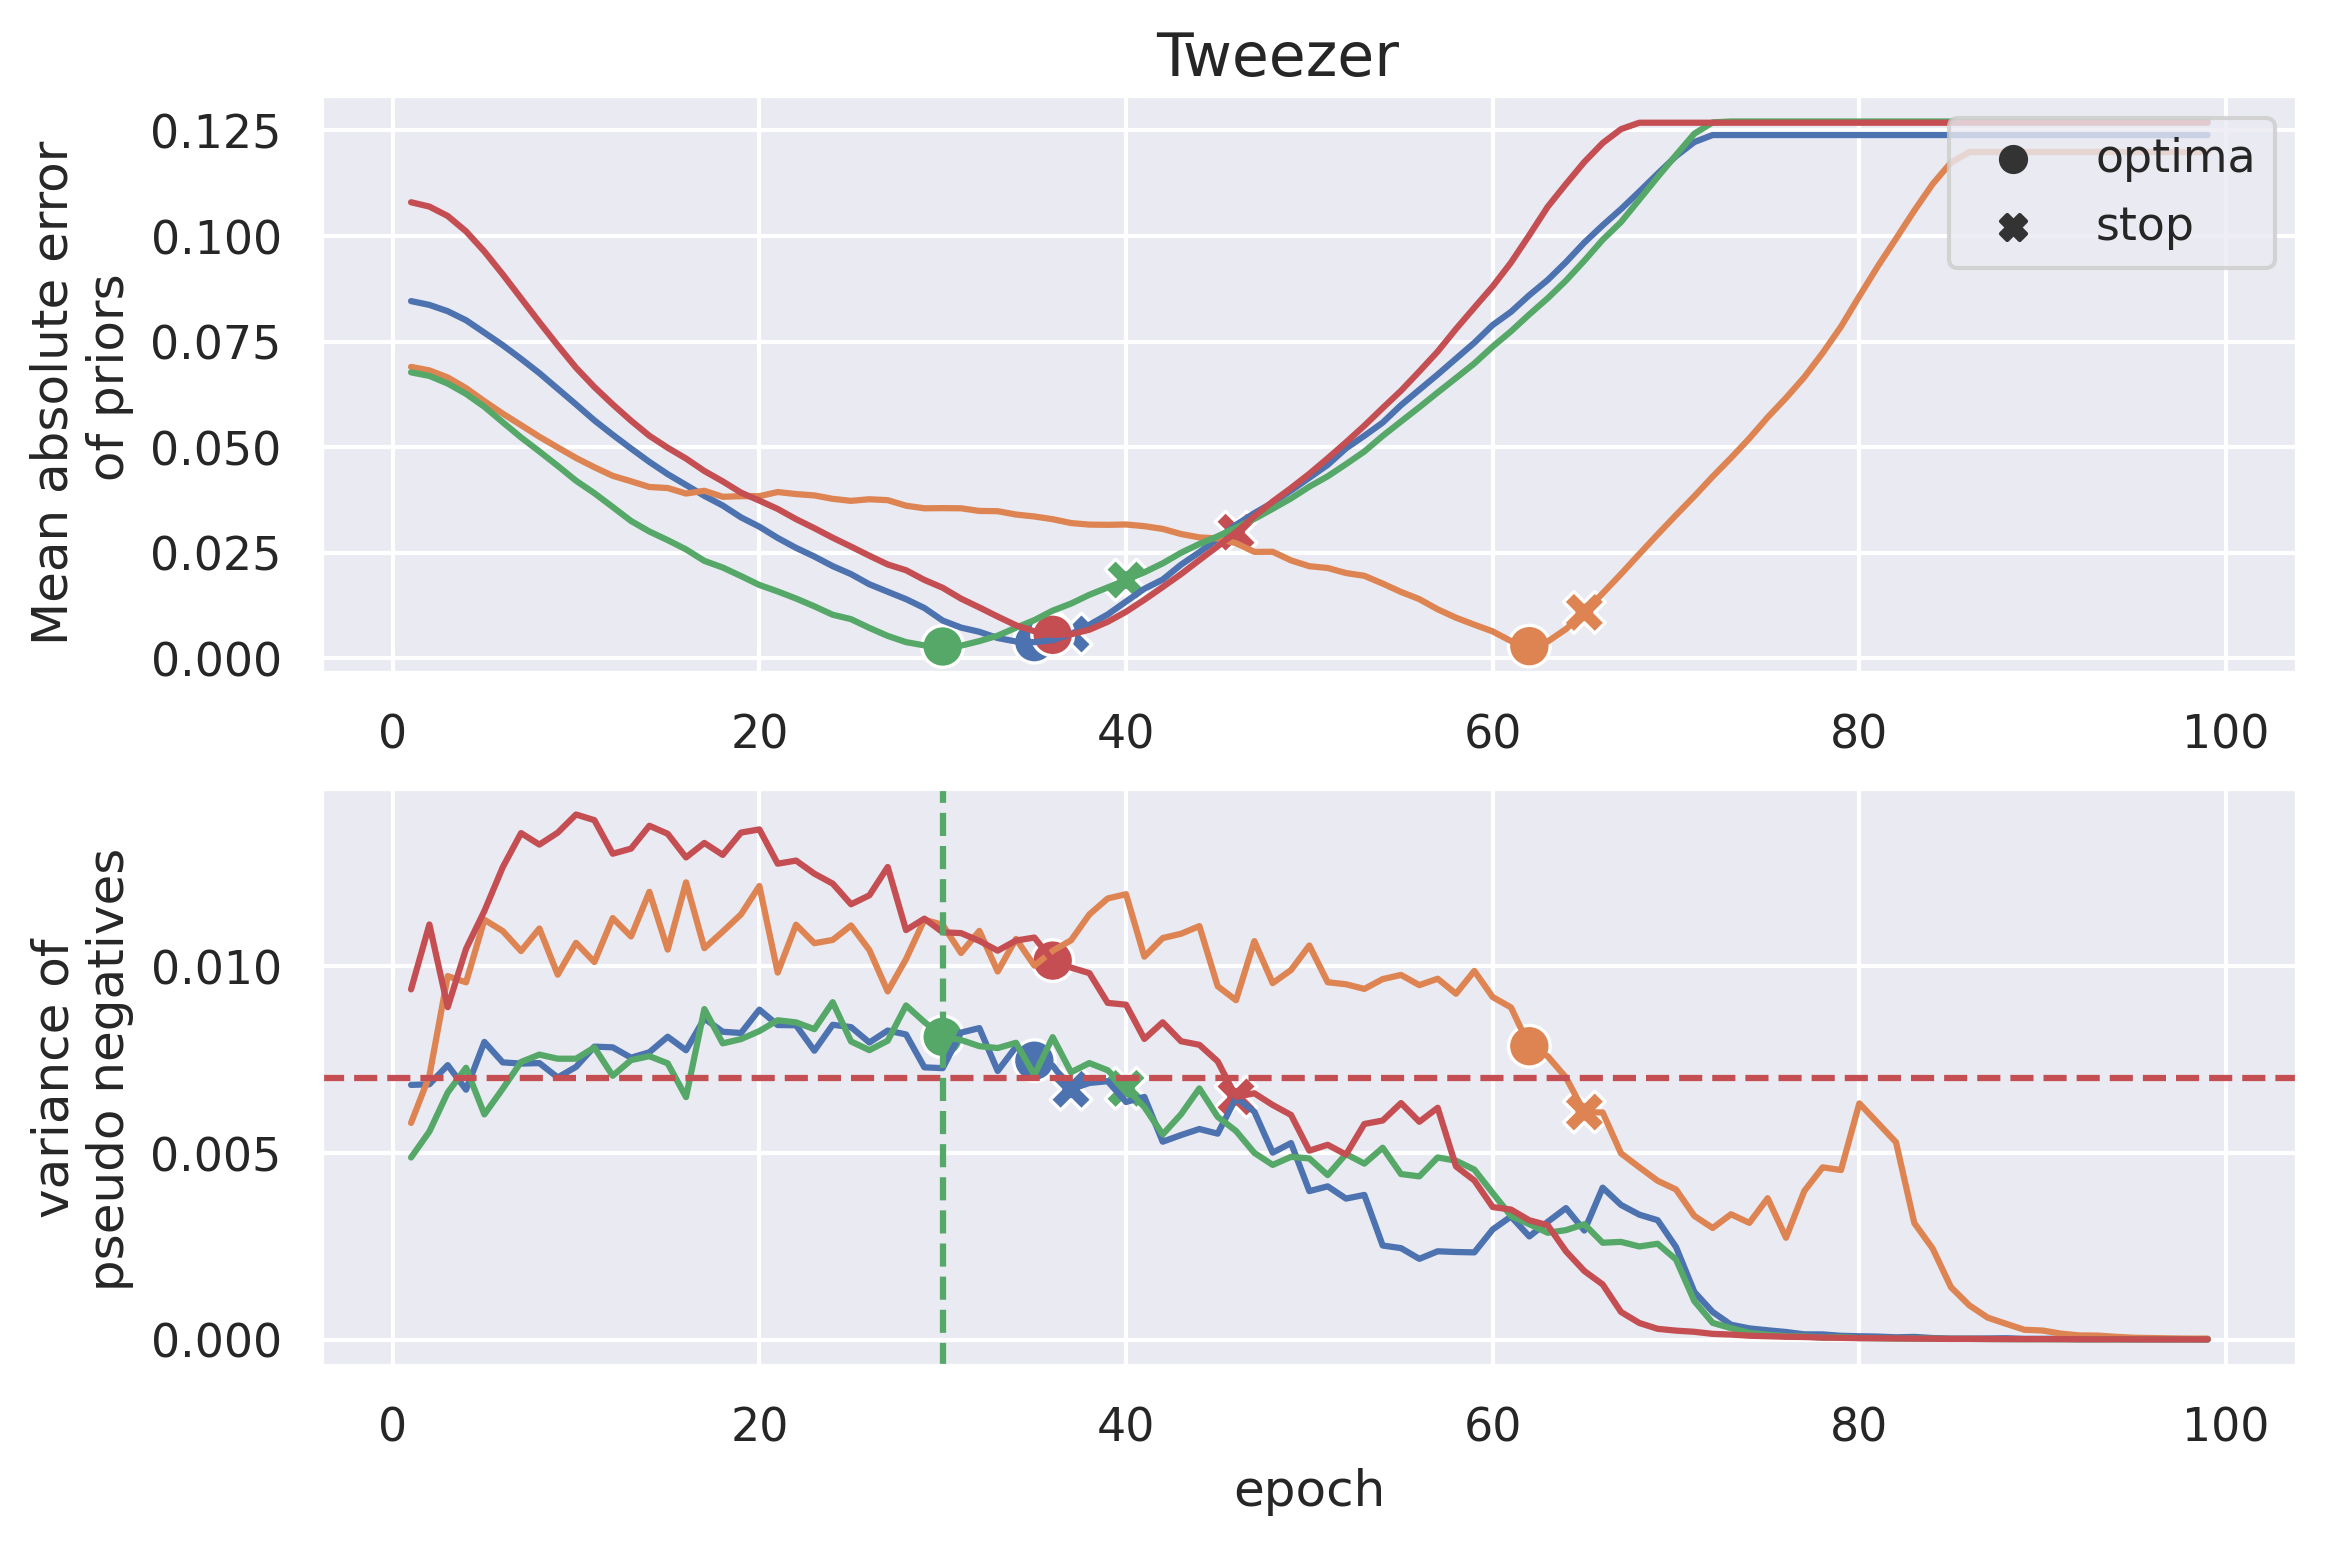
\includegraphics[width=.5\textwidth]{tweezer_priors.png} &
    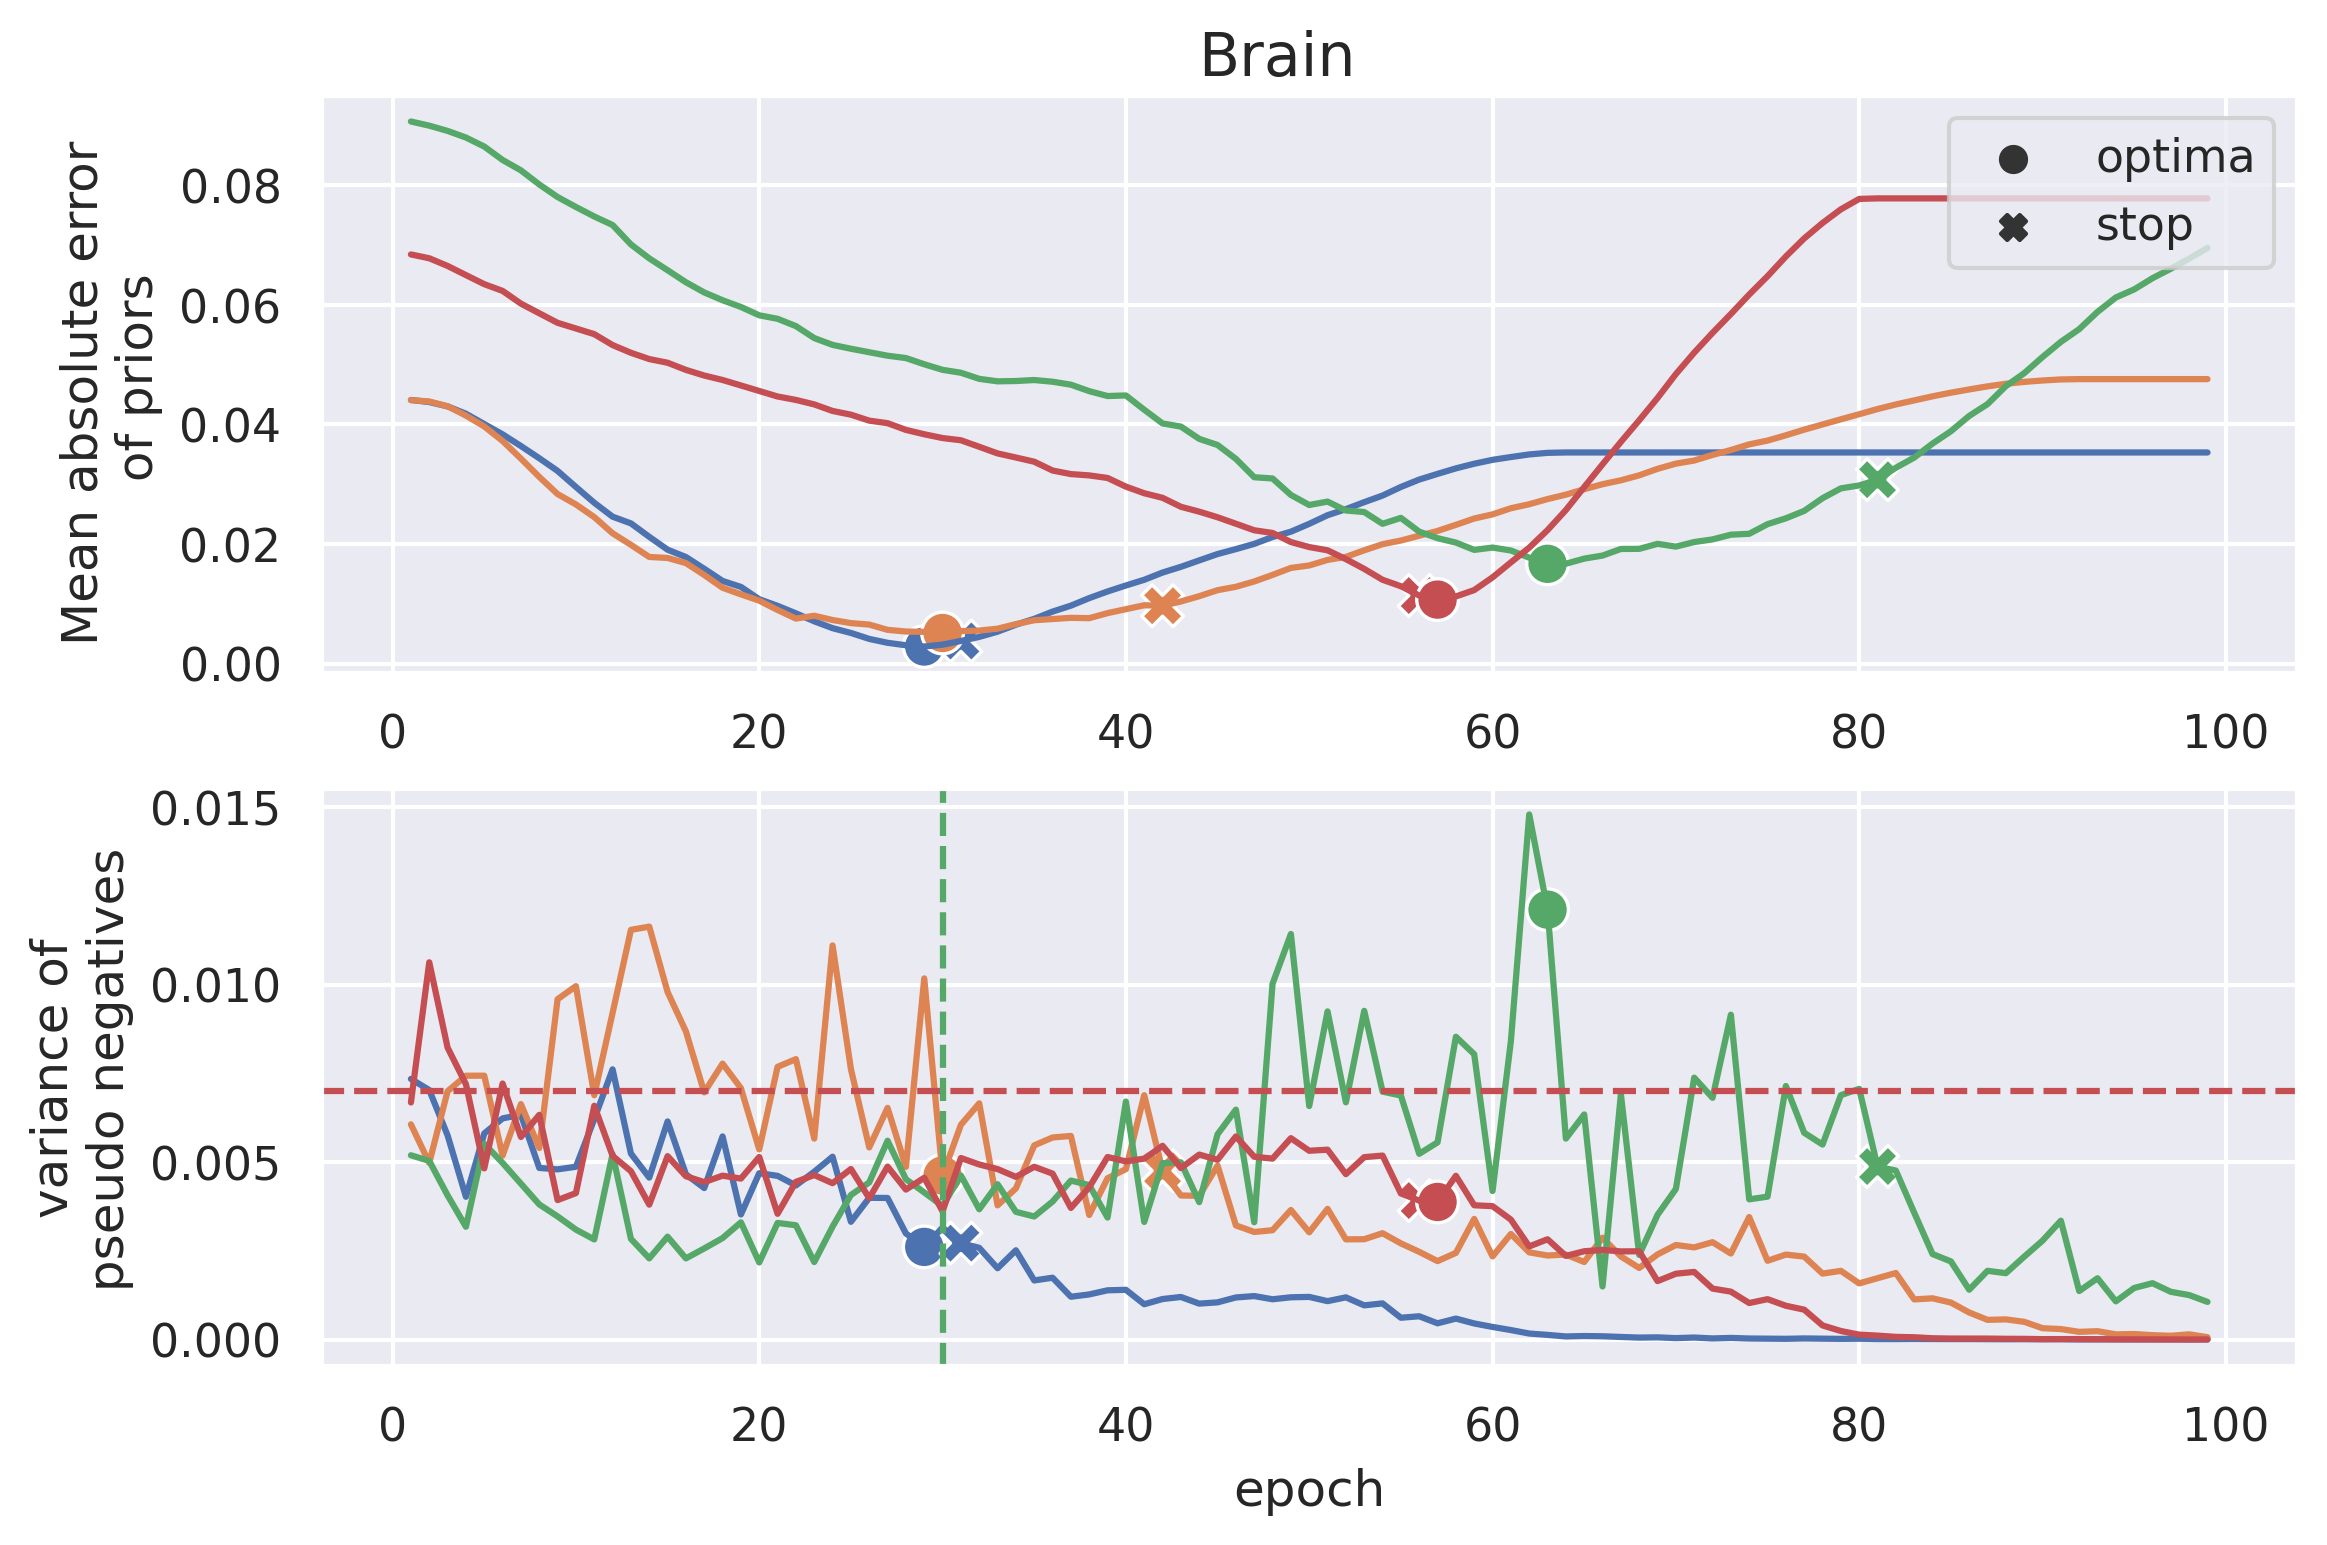
\includegraphics[width=.5\textwidth]{brain_priors.png} \\
    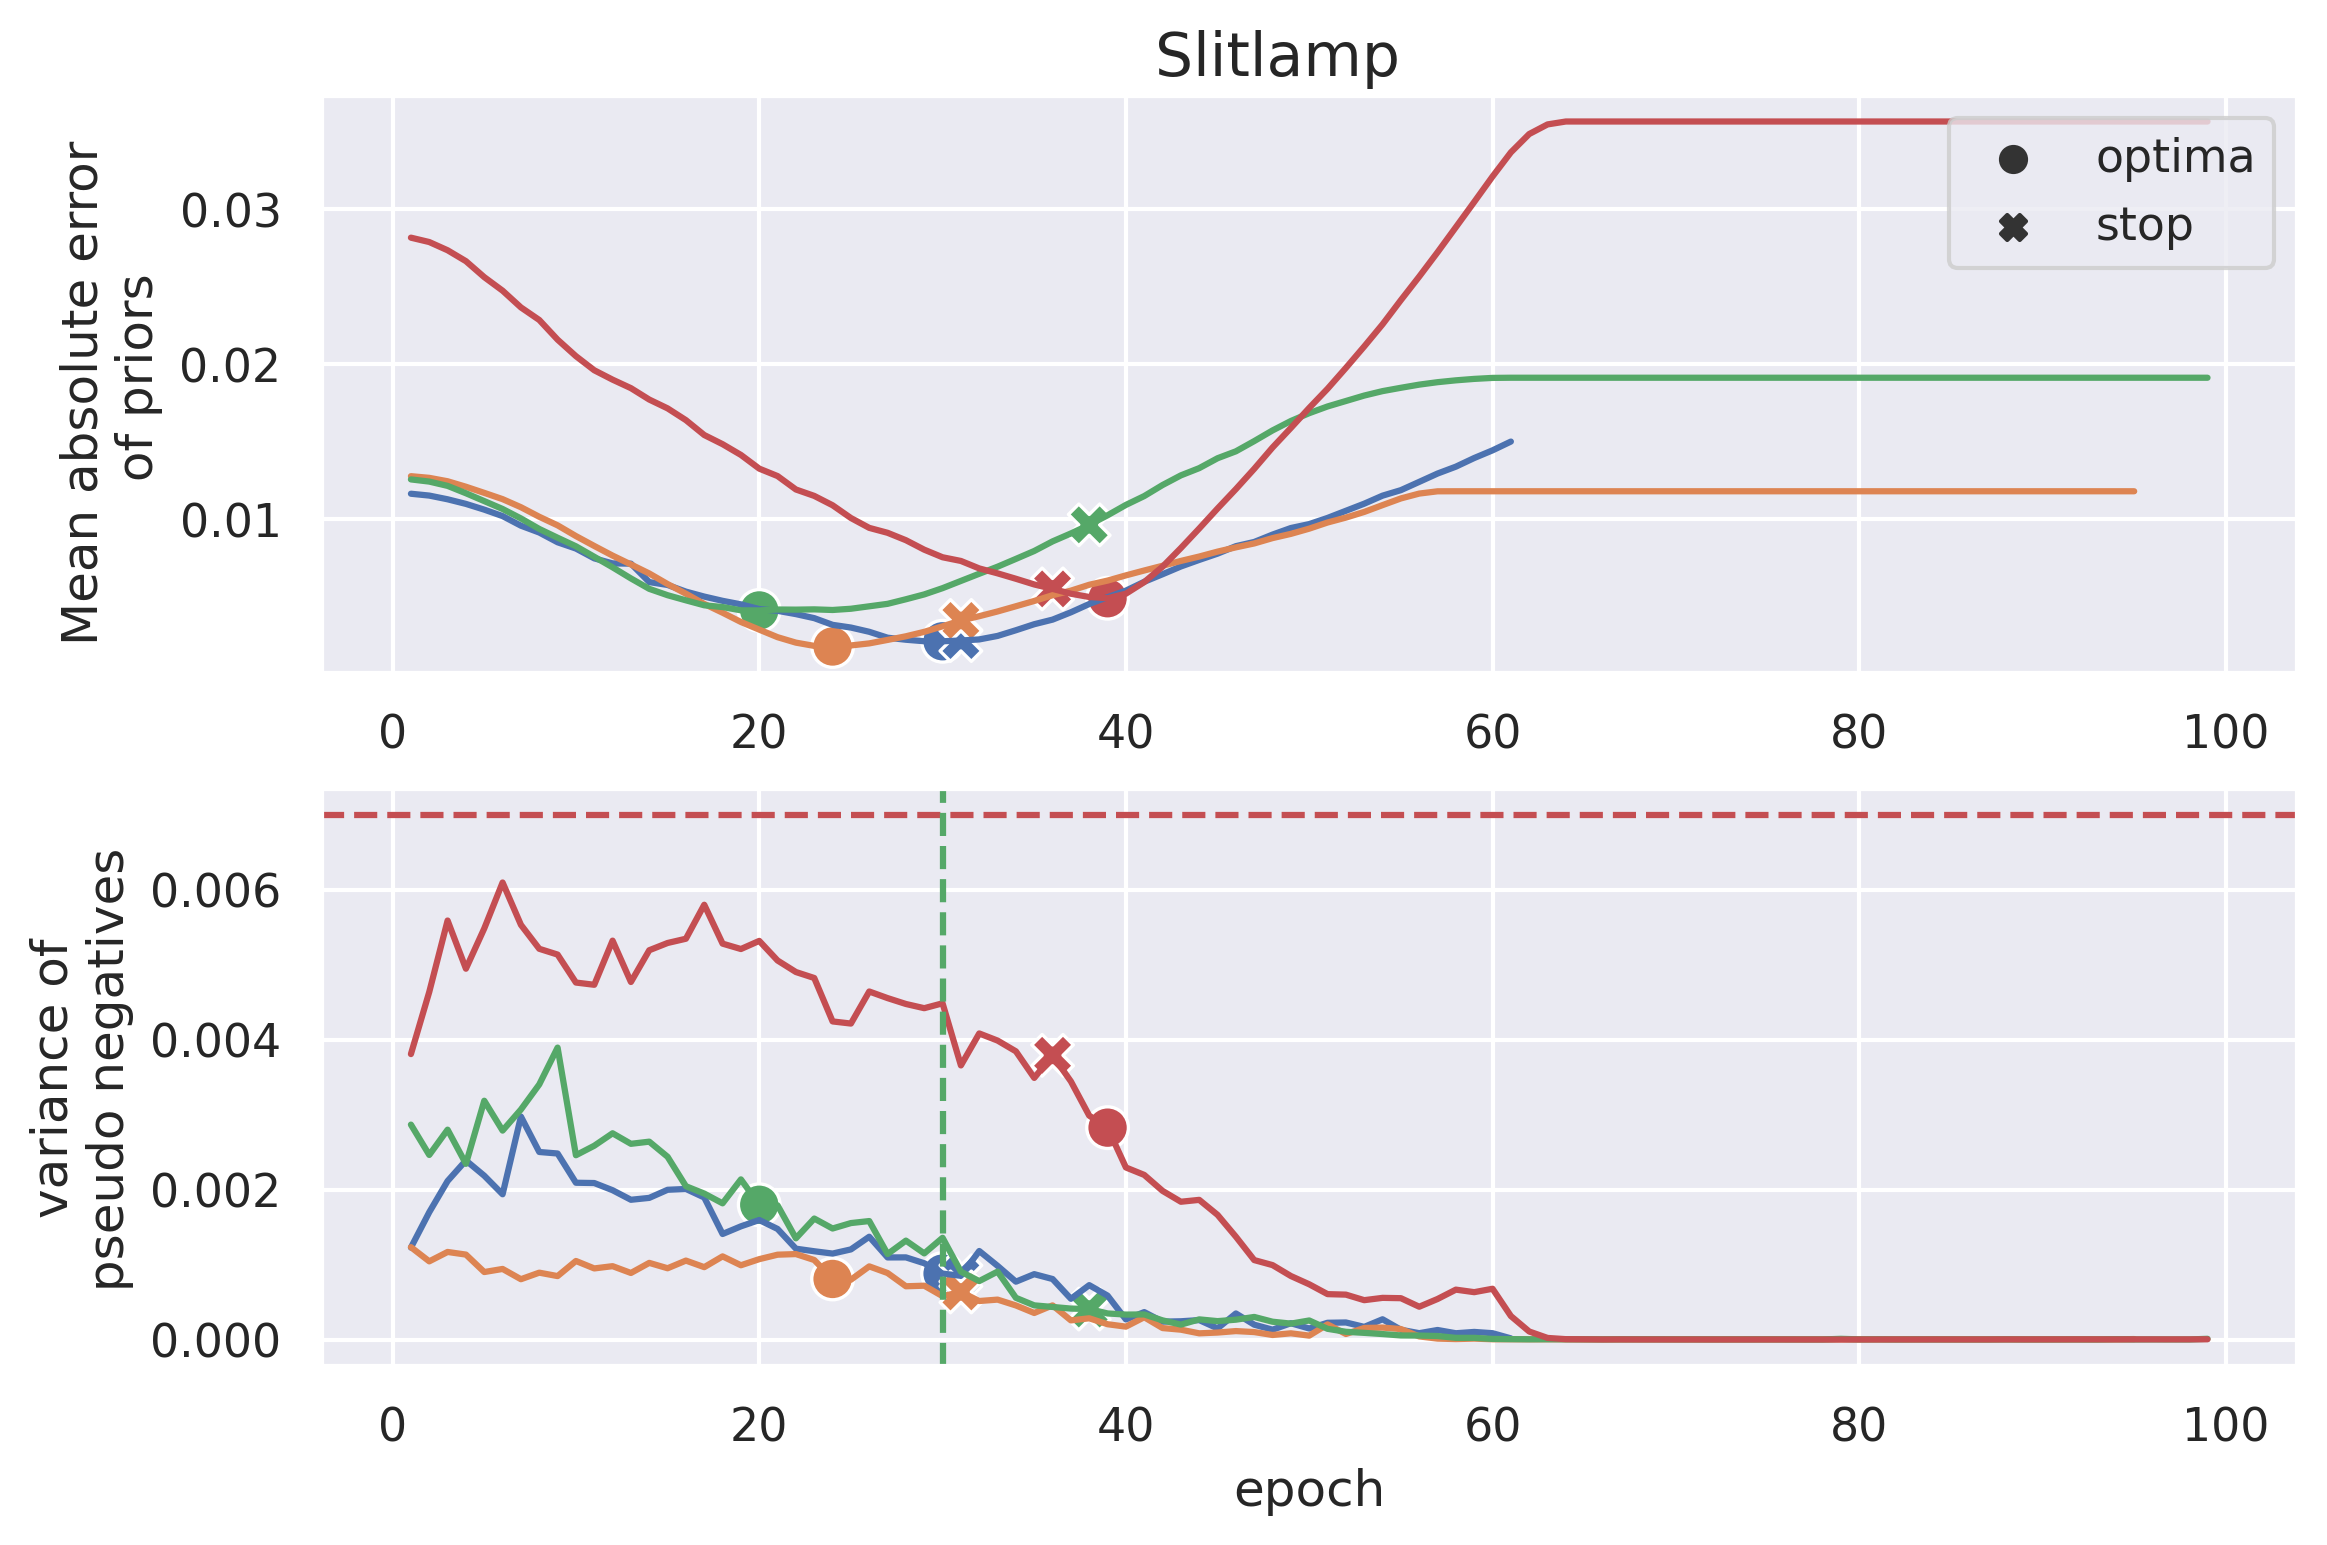
\includegraphics[width=.5\textwidth]{slitlamp_priors.png} &
    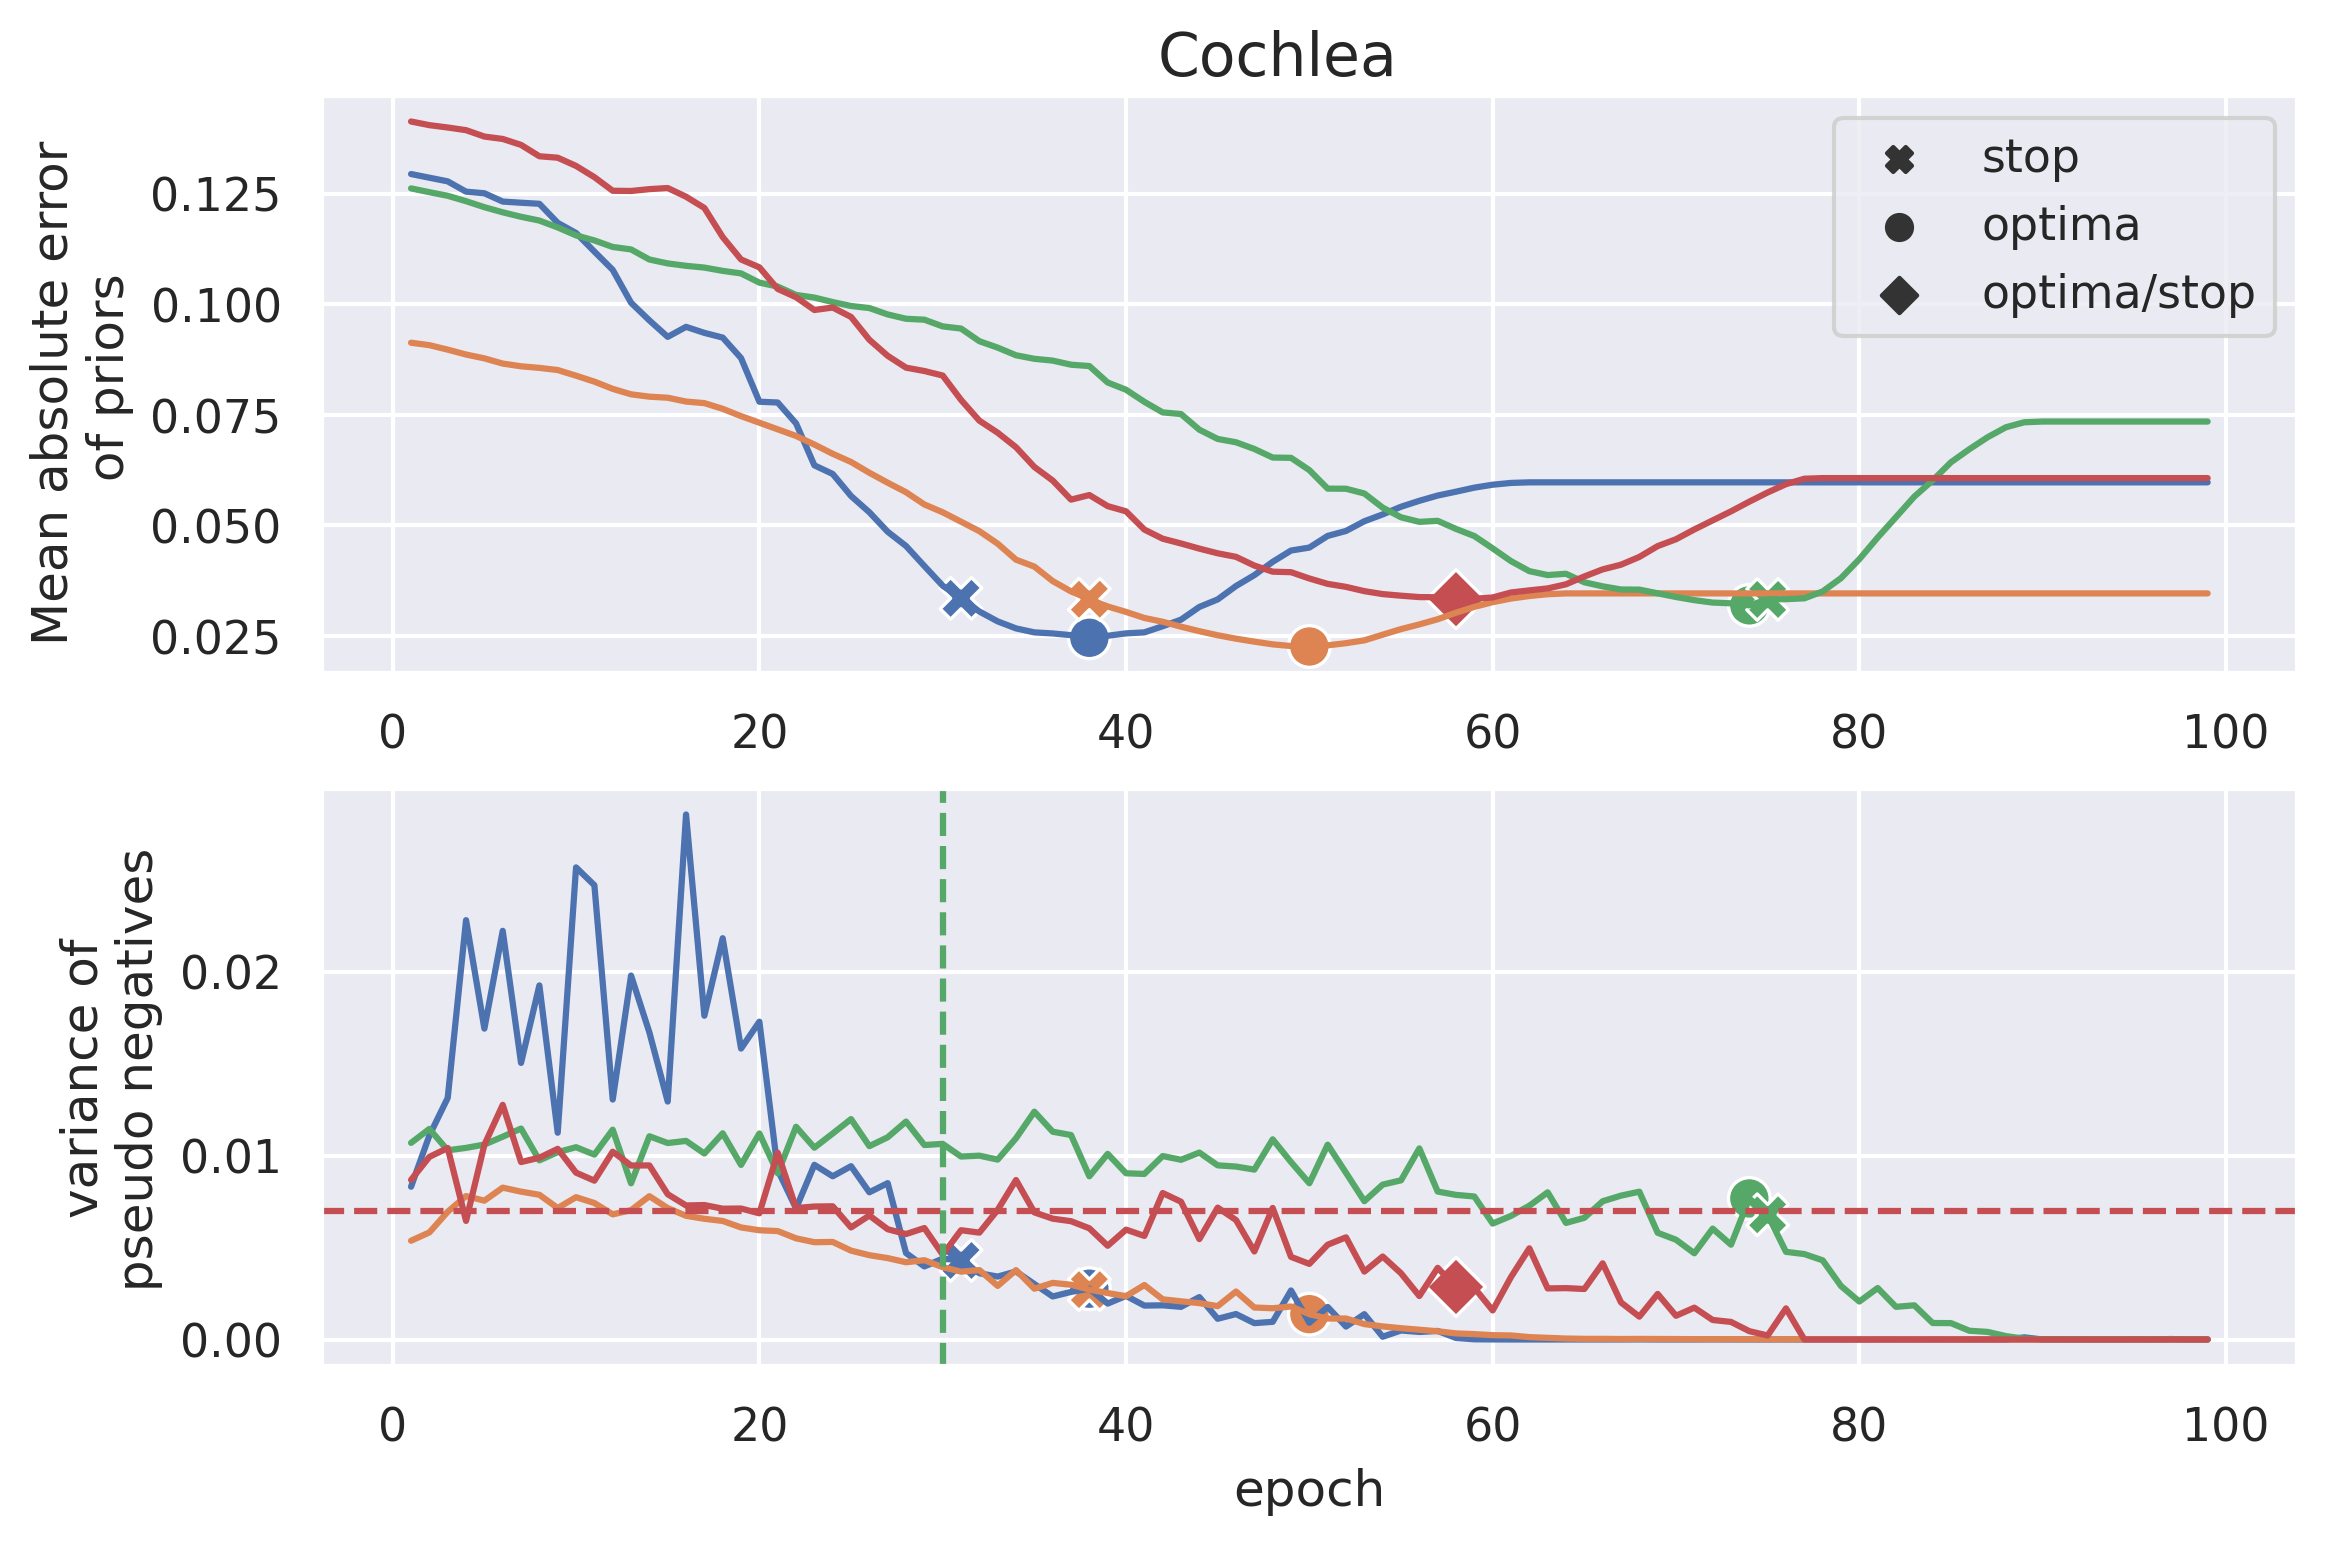
\includegraphics[width=.5\textwidth]{cochlea_priors.png} \\
\end{tabular}
\label{fig:converge}
\end{figure*}

\subsection{Segmentation performance}
\label{sec:exp_performance}
Using the datasets mentioned above, we evaluate the proposed methods (\SSnnPU~and \SSnnPUKSP) quantitatively and qualitatively. Additionally, we compare these to existing methods that perform the same tasks. These include:
\begin{itemize}
\item \KSPTrack: Multi-object tracking method described in \cite{lejeune18}. As in the original work, the object model consists of a decision tree bagger adapted to the PU setting, while features are taken from a CNN configured as an autoencoder.
\item \textbf{EEL}: An expected exponential loss within a boosting framework for robust classication in a PU learning setting~\cite{lejeune17}.
\item \textbf{Gaze2Segment}: A learned saliency-map based detection regularized with graphcut~\cite{khosravan16}.
\item \textbf{DL-prior}: Point location supervision is used to train a CNN with strong object priors~\cite{bearman16}.
\end{itemize}

For our method, we set the initial class prior upper-bound, $\pi_{max}$, by computing the frequencies of positives $\pi^{i}$ for all frames from the groundtruth and set $\hat \pi_{0}=1.4 \cdot \max_{i} \{ \pi^{i} \}$. While this may appear to be using the groundtruth to set the parameters of our method, it allows us to calibrate $\pi$ for comparison reasons. Indeed, a 40\% factor over the frame that has the largest object surface object can represent the entire image depending on the dataset. To show that our method is not inherently sensitive to this value, we perform an analysis of sensitivity in Sec.~\ref{sec:ablation}.
\begin{table*}[t]
\centering
\caption{
    Quantitative results on all datasets. We report the F1 scores and standard deviations.
    }
\label{tab:results}
\begin{tabular}{llp{1.8cm}p{1.8cm}p{1.8cm}p{1.8cm}p{1.8cm}}
\toprule
Types &               Tweezer &               Cochlea &              Slitlamp &                Brain \\
Methods         &                       &                       &                       &                      \\
\midrule
KSPTrack/nnPUss &  $\bm{0.91} \pm 0.03$ &  $\bm{0.75} \pm 0.05$ &  $\bm{0.84} \pm 0.05$ &  $\bm{0.8} \pm 0.09$ \\
nnPUss          &       $0.87 \pm 0.02$ &        $0.53 \pm 0.1$ &        $0.78 \pm 0.1$ &      $0.75 \pm 0.13$ \\
\hdashline
KSPTrack        &       $0.77 \pm 0.08$ &       $0.66 \pm 0.02$ &       $0.77 \pm 0.08$ &      $0.74 \pm 0.08$ \\
EEL             &        $0.6 \pm 0.16$ &       $0.12 \pm 0.05$ &       $0.59 \pm 0.08$ &      $0.52 \pm 0.14$ \\
Gaze2Segment    &        $0.18 \pm 0.0$ &       $0.07 \pm 0.02$ &        $0.02 \pm 0.0$ &      $0.07 \pm 0.02$ \\
DL-prior        &       $0.72 \pm 0.06$ &        $0.3 \pm 0.04$ &       $0.51 \pm 0.11$ &      $0.56 \pm 0.08$ \\
\bottomrule
\end{tabular}
\end{table*}


\begin{figure*}[t]
\caption{Qualitative results for each type. From left to right: Original image with groundtruth highlighted in red and 2D location in green, output of foreground prediction model (SSnnPU), SSnnPU combined with our spatio-temporal regularization scheme (SSnnPU+KSPTrack), best baseline (KSPTrack), and second best baseline (EEL).}
\centering
    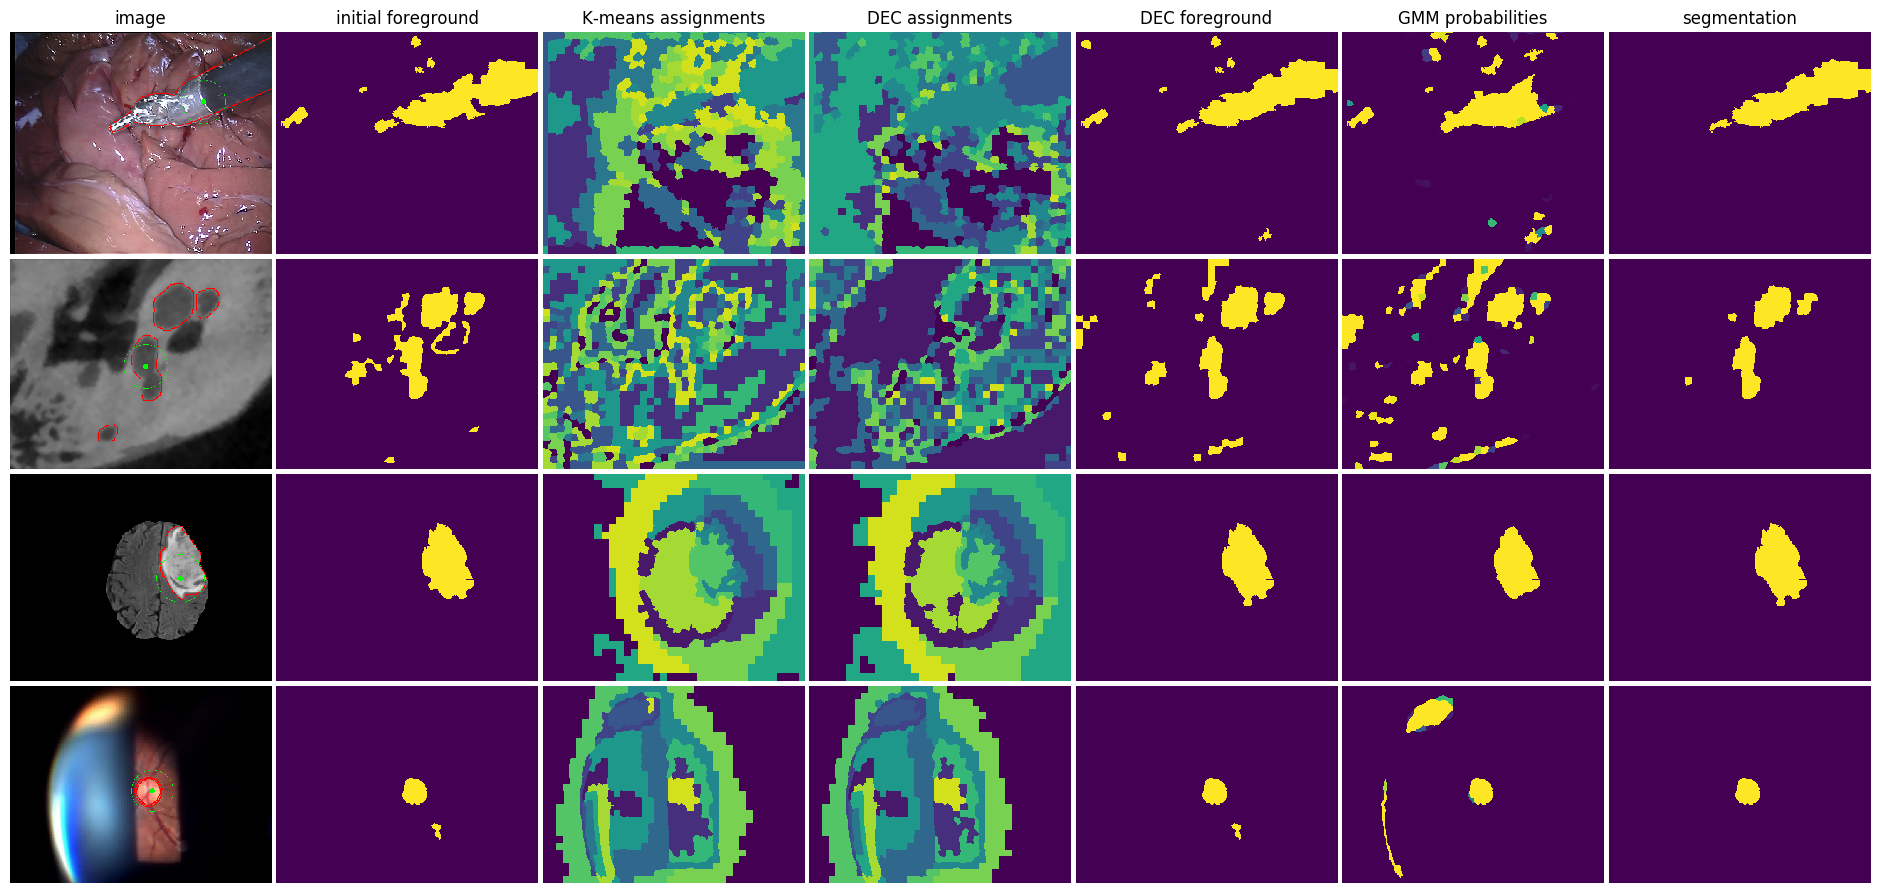
\includegraphics[width=.65\textwidth]{prevs.png}
\label{fig:prevs}
\end{figure*}

In Table.~\ref{tab:results}, we show the F1 scores of each method, averaged over each sequence for each data type. Given that some methods require superpixels, we also show the maximum performance a segmentation method would have if every single superpixel was correctly labeled. In practice we denote positive superpixels as those with more than half of the pixels are in the groundtruth. We then compare the latter segmentation with the pixel-wise manual ground truth annotation and denote the result \MaxSP.

From these results, we note that both \SSnnPU~and \SSnnPUKSP~ perform well on average. Most notably, \SSnnPUKSP~outperformes all other approaches including \SSnnPU. This is coherent as the spatio-temporal regularization provides an efficient method to remove false positives generated by \SSnnPU. On the Tweezer sequences, the gain in performances are striking, with an increase in 14\% on average over the previous state-of-the-art, and closely approaches a perfect labeling according to \MaxSP.

When comparing \SSnnPU~and \SSnnPUKSP, we note that the spatio-temporal regularization provided by the KSP is particularly effective in the Cochlea cases (\ie plus 18\%). This is coherent as the geometry of the cochlea is largely made of a rings and where visual appearance plays a somewhat lesser role in identifying the complete structure. This latter point also explains the fairly poor performance of \SSnnPU~but much improved one by \SSnnPUKSP~when compared to \KSPTrack. 

In Fig.~\ref{fig:prevs}, we show qualitative results of different methods and provide complete video results of \SSnnPUKSP~ as supplementary material.

\subsection{Ablation study}
\label{sec:ablation}
To provide a better understanding as to what aspects of our method provide improvements, we perform an ablation study. Specifically, we evaluate the following variants of our methods:
\begin{itemize}
\item \SSnnPU: Non-negative positive-unlabeled with self-supervised class-prior estimation, as in Sec.~\ref{sec:nnpu} and~\ref{sec:pi_estim}.
\item \SSnnPUKSP: Combines the \SSnnPU~method and the \KSPTrack~methods described in Sec.~\ref{sec:tracking}.
\item \SSnnPUTrue: Same as \SSnnPUKSP, except that the foreground model is directly trained using the true class-priors (\ie. taken from the groundtruth) following Alg.~\ref{alg:sgdnnpu}.
\item \SSnnPUConst: Same as \SSnnPUTrue, except that we use a sequence-wise constant class prior given by the mean groundtruth prior over all frames (as in~\cite{kiryo17}).
\end{itemize}
For both \SSnnPUTrue~and \SSnnPUConst, we train the models $f$ for $150$ epochs. The learning rate in both cases are set to $10^{-4}$ and reduced to $10^{-5}$ after $50$ epochs.

\begin{table*}
\centering
\caption{
    Quantitative results on all datasets for different prior levels. We report the F1 score, precision (PR), recall(RC) and standard deviations.
    }
\label{tab:results_eta}
\begin{tabular}{llp{1.8cm}p{1.8cm}p{1.8cm}p{1.8cm}}
\toprule
      &                   &   &              F1 &              PR &              RC \\
Types & Methods & $\eta$ &                 &                 &                 \\
\midrule
\multirow{9}{*}{Tweezer} & \multirow{4}{*}{nnPUconst+KSPTrack} & 0.8 &  $0.89\pm 0.03$ &  $0.91\pm 0.05$ &  $0.88\pm 0.03$ \\
      &                   & 1.0 &  $0.90\pm 0.04$ &  $0.86\pm 0.06$ &  $0.93\pm 0.02$ \\
      &                   & 1.2 &  $0.90\pm 0.03$ &  $0.84\pm 0.05$ &  $0.96\pm 0.01$ \\
      &                   & 1.4 &  $0.89\pm 0.03$ &  $0.83\pm 0.05$ &  $0.97\pm 0.00$ \\
\cline{2-6}
      & \multirow{4}{*}{nnPUss+KSPTrack} & 1.2 &  $0.92\pm 0.01$ &  $0.93\pm 0.02$ &  $0.92\pm 0.03$ \\
      &                   & 1.4 &  $0.91\pm 0.03$ &  $0.91\pm 0.03$ &  $0.91\pm 0.05$ \\
      &                   & 1.6 &  $0.91\pm 0.03$ &  $0.88\pm 0.03$ &  $0.94\pm 0.03$ \\
      &                   & 1.8 &  $0.90\pm 0.04$ &  $0.88\pm 0.04$ &  $0.92\pm 0.04$ \\
\cline{2-6}
      & nnPUtrue+KSPTrack & - &  $0.90\pm 0.03$ &  $0.89\pm 0.03$ &  $0.92\pm 0.04$ \\
\cline{1-6}
\multirow{9}{*}{Cochlea} & \multirow{4}{*}{nnPUconst+KSPTrack} & 0.8 &  $0.59\pm 0.15$ &  $0.88\pm 0.09$ &  $0.45\pm 0.15$ \\
      &                   & 1.0 &  $0.67\pm 0.07$ &  $0.87\pm 0.14$ &  $0.55\pm 0.06$ \\
      &                   & 1.2 &  $0.71\pm 0.10$ &  $0.91\pm 0.10$ &  $0.59\pm 0.12$ \\
      &                   & 1.4 &  $0.68\pm 0.10$ &  $0.77\pm 0.18$ &  $0.62\pm 0.11$ \\
\cline{2-6}
      & \multirow{4}{*}{nnPUss+KSPTrack} & 1.2 &  $0.73\pm 0.08$ &  $0.85\pm 0.16$ &  $0.65\pm 0.03$ \\
      &                   & 1.4 &  $0.75\pm 0.05$ &  $0.88\pm 0.08$ &  $0.66\pm 0.04$ \\
      &                   & 1.6 &  $0.72\pm 0.07$ &  $0.80\pm 0.20$ &  $0.68\pm 0.07$ \\
      &                   & 1.8 &  $0.64\pm 0.14$ &  $0.80\pm 0.32$ &  $0.58\pm 0.07$ \\
\cline{2-6}
      & nnPUtrue+KSPTrack & - &  $0.76\pm 0.05$ &  $0.85\pm 0.08$ &  $0.69\pm 0.03$ \\
\cline{1-6}
\multirow{9}{*}{Slitlamp} & \multirow{4}{*}{nnPUconst+KSPTrack} & 0.8 &  $0.71\pm 0.30$ &  $0.84\pm 0.08$ &  $0.72\pm 0.38$ \\
      &                   & 1.0 &  $0.84\pm 0.03$ &  $0.79\pm 0.05$ &  $0.91\pm 0.04$ \\
      &                   & 1.2 &  $0.78\pm 0.05$ &  $0.66\pm 0.07$ &  $0.95\pm 0.01$ \\
      &                   & 1.4 &  $0.66\pm 0.04$ &  $0.51\pm 0.05$ &  $0.95\pm 0.01$ \\
\cline{2-6}
      & \multirow{4}{*}{nnPUss+KSPTrack} & 1.2 &  $0.72\pm 0.29$ &  $0.92\pm 0.05$ &  $0.67\pm 0.34$ \\
      &                   & 1.4 &  $0.84\pm 0.05$ &  $0.85\pm 0.08$ &  $0.84\pm 0.12$ \\
      &                   & 1.6 &  $0.80\pm 0.11$ &  $0.89\pm 0.06$ &  $0.75\pm 0.19$ \\
      &                   & 1.8 &  $0.84\pm 0.04$ &  $0.77\pm 0.06$ &  $0.92\pm 0.02$ \\
\cline{2-6}
      & nnPUtrue+KSPTrack & - &  $0.84\pm 0.03$ &  $0.79\pm 0.04$ &  $0.90\pm 0.02$ \\
\cline{1-6}
\multirow{9}{*}{Brain} & \multirow{4}{*}{nnPUconst+KSPTrack} & 0.8 &  $0.79\pm 0.09$ &  $0.82\pm 0.18$ &  $0.78\pm 0.04$ \\
      &                   & 1.0 &  $0.78\pm 0.11$ &  $0.77\pm 0.12$ &  $0.79\pm 0.10$ \\
      &                   & 1.2 &  $0.72\pm 0.09$ &  $0.60\pm 0.10$ &  $0.92\pm 0.06$ \\
      &                   & 1.4 &  $0.73\pm 0.08$ &  $0.60\pm 0.09$ &  $0.93\pm 0.06$ \\
\cline{2-6}
      & \multirow{4}{*}{nnPUss+KSPTrack} & 1.2 &  $0.79\pm 0.10$ &  $0.82\pm 0.14$ &  $0.76\pm 0.07$ \\
      &                   & 1.4 &  $0.80\pm 0.09$ &  $0.78\pm 0.14$ &  $0.84\pm 0.07$ \\
      &                   & 1.6 &  $0.77\pm 0.10$ &  $0.80\pm 0.12$ &  $0.75\pm 0.12$ \\
      &                   & 1.8 &  $0.76\pm 0.11$ &  $0.80\pm 0.11$ &  $0.73\pm 0.17$ \\
\cline{2-6}
      & nnPUtrue+KSPTrack & - &  $0.80\pm 0.09$ &  $0.73\pm 0.10$ &  $0.89\pm 0.07$ \\
\bottomrule
\end{tabular}
\end{table*}


In addition, to assess how \SSnnPUKSP~performs as a function of the selected $\pi_{max}$, we evaluate the method using $\hat \pi_{0}=\eta \max_{i}\pi^{i}$, with $\eta \in \{1.2, 1.4, 1.6, 1.8\}$. Similarly, to assess the relevance of the self-supervised estimation of priors, we perform segmentation using method \SSnnPUConst~with $\eta \in \{0.8, 1.0, 1.2, 1.4\}$.

We report F1, precision and recall scores for each aforementioned method in Table.~\ref{tab:results_eta}. First, we observe that our self-supervised estimation is relatively robust to variations in $\hat \pi_{0}$.
In particular, Tweezer shows variations in F1 scores of at most $1\%$ while $\eta$ ranges between $1.2$ and $1.6$. Similarly, the performances fluctuate only marginally for Cochlea, Slitlamp and Brain sequences with at most 5\% changes. These fluctuations still lead to improved performances over state-of-the-art methods.

In contrast, sensitivity to initial class priors is much stronger for \SSnnPUConst, which yields variations between 1\% and 15\% depending on the sequence type. The relevance of the frame-wise prior estimation can also be assessed by comparing, for each sequence type, the maximum F1 scores reached by \SSnnPUKSP~and \SSnnPUConst~for all tested values of $\eta$. \SSnnPUKSP~brings an improvement over \SSnnPUConst~of $2\%, 1\%, 6\%$ and $0\%$ for the Tweezer, Brain, Cochlea and Slitlamp sequence, respectively.

Last, comparing \SSnnPUKSP~to \SSnnPUTrue, we note that the proposed self-supervised prior estimation framework brings comparable performances on all types. That is the \SSnnPU~ component of our methods appears to provide class priors on par with the true class-priors. Surprisingly, in the Tweezer case, some values of $\eta$ yield even better performances than if the true class prior values were to be used.


\subsection{Analysis of Convergence}
\label{sec:convergence}

Last, we analyze the behavior of our proposed stopping conditions in Alg.~\ref{alg:prior_estim}. In particular, Fig.~\ref{fig:converge} illustrates the convergence of the class prior estimation for each type of sequence. In these cases, all sequences are trained using $\hat\pi_{0}= 1.4 \cdot \max_i \{\pi^i\}$.

As we aim to estimate the true class-prior, we plot the Mean Absolute Error between the estimated priors and the true priors (top panels).
The proposed stopping condition, which leverages the variance of pseudo-negatives, is plotted in the bottom panel. We observe that the proposed stopping condition triggers reasonably close to the optima in most cases. In cases where the stopping condition is triggered earlier or later, we note that the difference in mean absolute error is fairly small, whereby implying that the impact in the early/late trigger is rather small. 


%%% Local Variables:
%%% mode: latex
%%% TeX-master: "main"
%%% End:
